\documentclass[dcc]{fcfmcourse}
\usepackage{teoria}
\usepackage[utf8x]{inputenc}
\usepackage{amsmath}
\usepackage{amsfonts,setspace}
\usepackage{listings}
\usepackage{color}
\usepackage{cancel}
\usepackage{epstopdf}
\usepackage{qtree}
\usepackage{fancyhdr}
\usepackage{tikz}
\usepackage{hyperref}
\usetikzlibrary{automata,positioning}
\pagestyle{fancy}
\cfoot{``Those who can imagine anything, can create the impossible." \\Alan Turing}
\definecolor{pblue}{rgb}{0.13,0.13,1}
\definecolor{pgreen}{rgb}{0,0.5,0}
\definecolor{porange}{rgb}{0.9,0.5,0}
\definecolor{pgrey}{rgb}{0.46,0.45,0.48}

\lstset{language=Java,
  showspaces=false,
  showtabs=false,
  breaklines=true,
  showstringspaces=false,
  breakatwhitespace=true,
  commentstyle=\color{porange},
  keywordstyle=\color{pblue},
  stringstyle=\color{pgreen},
  basicstyle=\ttfamily,
  moredelim=[il][\textcolor{pgrey}]{$ $},
  moredelim=[is][\textcolor{pgrey}]{\%\%}{\%\%}
}

\newenvironment{codebox} {\small \ttfamily \obeylines \begingroup \setstretch{-2.4}} {\endgroup}

\title{Auxiliar 9}
\course[CC3102]{Teoría de la Computación}
\professor{Gonzalo Navarro}
\assistant{Manuel Cáceres}
\assistant{Ian Letter}

% Si pasas el comando usedate a la clase, la fecha aparecerá bajo la lista de auxiliares.
% Puedes usar el formato de fecha por defecto de latex (y traducirla usando babel)
% o puedes escribir lo que quieras con el comando \date.
% \date{1 de Septiembre, 2015}

\begin{document}
\maketitle
\begin{center}
16 de Noviembre del 2016
\end{center}
\vspace{-1ex}
\begin{problems}
 \problem Para un valor $k$ fijo, considere el lenguaje $L_{k-pack}$ que contiene a todos los strings de la forma
\begin{align*}
    \#0^{n_{1}}\$0^{n_{2}}\$\ldots\$0^{n_{l}}\#0^{m}\underline{\#}
\end{align*}
tales que existe una manera de distribuir los elementos $n_{1},n_{2},\ldots,n_{l}$ en $k$ grupos de manera tal que la suma de cada grupo es a los más $m$. Construya una $MT$ que acepte a $L_{k-pack}$.
\problem El \textit{lenguaje de salida} de una $MT$ $M$ es:
\begin{align*}
   \{ w \in \left(\Sigma \setminus \{\#\}\right)^* ,\ \exists u \in \left(\Sigma \setminus \{\#\}\right)^*,\  \left(s,\# u\underline{\# }\right)\vdash_{M}^{*}\left(h,\# w\underline{\#}\right) \}
\end{align*}
Muestre que un lenguaje $L$ es aceptable sii es el \textit{lenguaje de salida} de alguna $MT$.
\problem Un lenguaje $L$ es \textit{enumerable} si existe una $MT$ $M=(K,\Sigma,\delta, s)$ y un estado $q \in K$ tal que
\begin{align*}
    L = \{ w\in \left(\Sigma \setminus \{\#\}\right)^*,\ \exists u \in \Sigma^*, \  \left(s,\underline{\# }\right)\vdash_{M}^{*}\left(q,\# w\underline{\#}u\right)\}
\end{align*}
Muestre que un lenguaje $L$ es enumerable sii es aceptable.
\problem Construya una $MT$ que acepte el lenguaje $\{0^{2^{n}}\colon n \ge 0\}$
\end{problems}
\newpage
\begin{center}
{\huge \underline{Soluciones}}
\end{center}
\begin{problems}
 \problem La idea es tener $k$ cintas doblemente infinitas adicionales. Luego por cada uno de los $0^{n_{i}}$'s elijo no deterministicamente copiarlo a alguna de estas cintas. Finalmente, reviso si se cumple la condición necesaria para estar en $L_{k-pack}$ (que todas las cintas tengan a lo más $m$ $0$'s). La $MTND$ es la siguiente:
 \begin{center}
 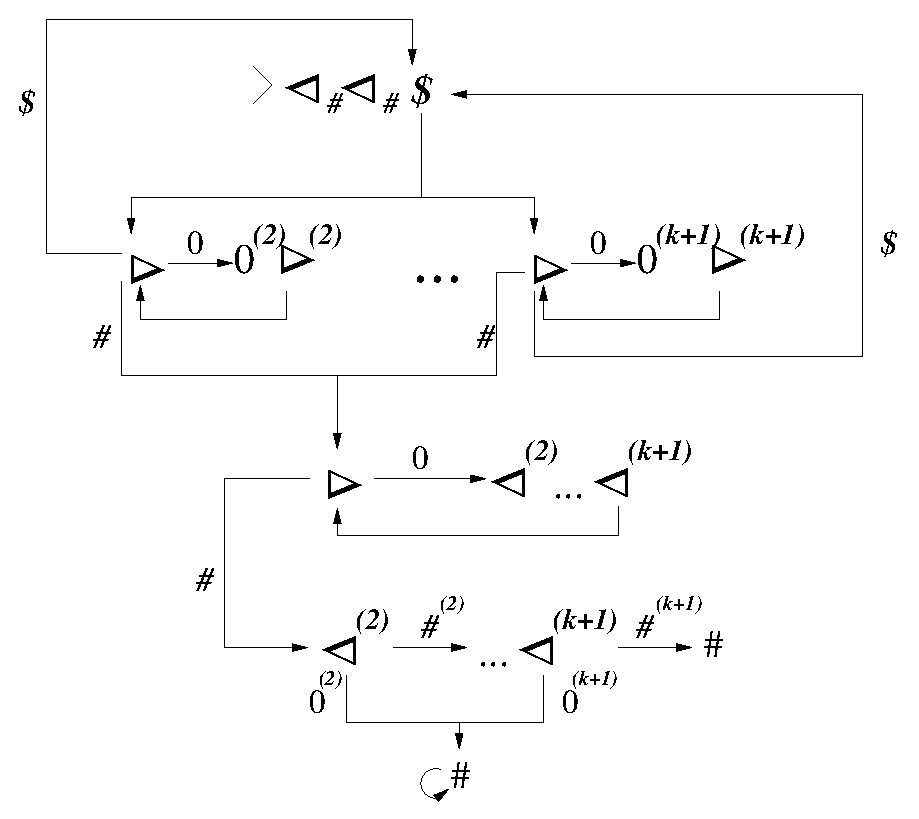
\includegraphics[scale=0.8]{9P12.eps}
 \end{center}
 \problem \textbf{Lema 5.8} del apunte \url{https://www.dcc.uchile.cl/~gnavarro/apunte.pdf}
 \problem \textbf{Lema 5.9} del apunte \url{https://www.dcc.uchile.cl/~gnavarro/apunte.pdf}
 \newpage
 \problem Con esta $MT$:
  \begin{center}
 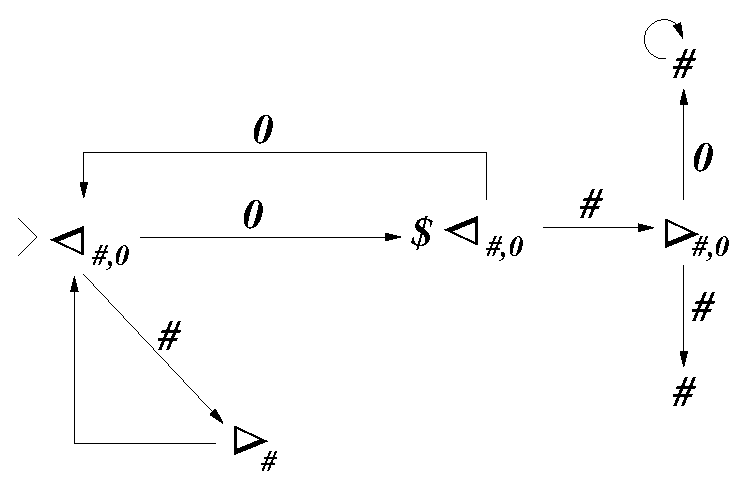
\includegraphics[scale=0.5]{9P4.eps}
 \end{center}
 Considerando $F$ como la máquina que computa $F(w) = ww$. $E$ como la máquina del \textbf{Ejemplo 4.11} del apunte \url{https://www.dcc.uchile.cl/~gnavarro/apunte.pdf} (que se detiene frente a las cadenas $\#w\#u\underline{\#}, w=u$ y $E_{D}$ como la máquina que \textit{decide} el lenguaje de las cadenas $\#w\#u\underline{\#}, w=u$.\footnote{Propuesto!}\\
 
 Cristóbal y Daniel propusieron esta $MT$:
 \begin{center}
 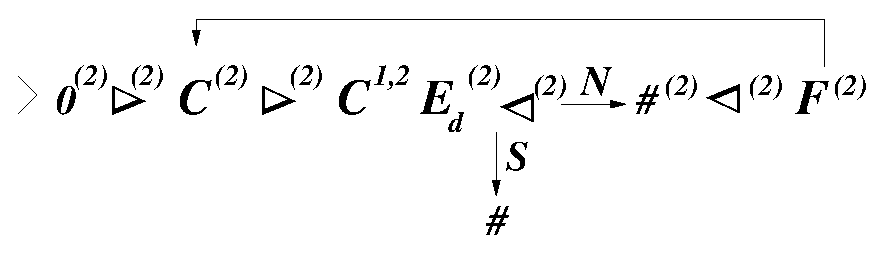
\includegraphics[scale=0.8]{9P42.eps}
 \end{center}
 Juan Pedro propuso una versión no determinista de lo anterior que es:
 \begin{center}
 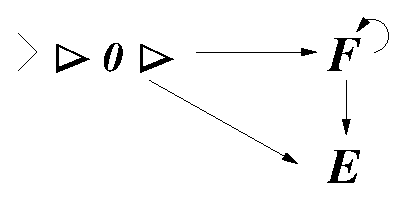
\includegraphics[scale=0.8]{9P43.eps}
 \end{center}
\end{problems}
\end{document}
